\subsection{Die Born-Näherung}
	Schrödingergleichung:
		\begin{align*}
			\left(- \frac{\hbar^2}{2 m} \vec{\nabla}^2 + V (\vec{r})\right) \phi
			&= \frac{\hbar^2 k^2}{2m} \phi \\
			\left(\vec{\nabla}^2 - k^2\right) \phi(\vec{r}) 
			&= \frac{2m}{\hbar^2} V (\vec{r}) \phi (\vec{r})
		\end{align*}
	Homogene Gleichung:
		\begin{align*}
			\left(\vec{\nabla}^2 + k^2 \right) \phi_0 (\vec{r}) = 0 &
			&(\text{Helmholzgleichung}) 
		\end{align*}
	Greenfunktion
		\begin{align*}
			\left(\vec{\nabla}^2 + k^2 \right) G (\vec{r} - \vec{r}\,') 
			&= \delta^{(3)}(\vec{r} - \vec{r}\,') \\
			G(\vec{r}) &= 
			\int \frac{\diff^3 q}{(2 \pi)^3} e^{i \vec{q} \cdot \vec{r}} \tilde{G}(\vec{q})
			&\text{mit } \tilde{G} (\vec{r}) &= \frac{1}{k^2-q^2} \\
			&= \int \frac{\diff^3 q}{(2 \pi)^3} \frac{e^{i \vec{q} \cdot \vec{r}}}{k^2 - q^2} \\
			&\underset{\text{E-Dynamik}}{=} - \frac{e^{\pm i k r}}{4 \pi r}
		\end{align*}
	$+$ steht für retadierte Lösung (Ursache vor Streuung)
	
	\begin{figure*} [h]
		\begin{center}
			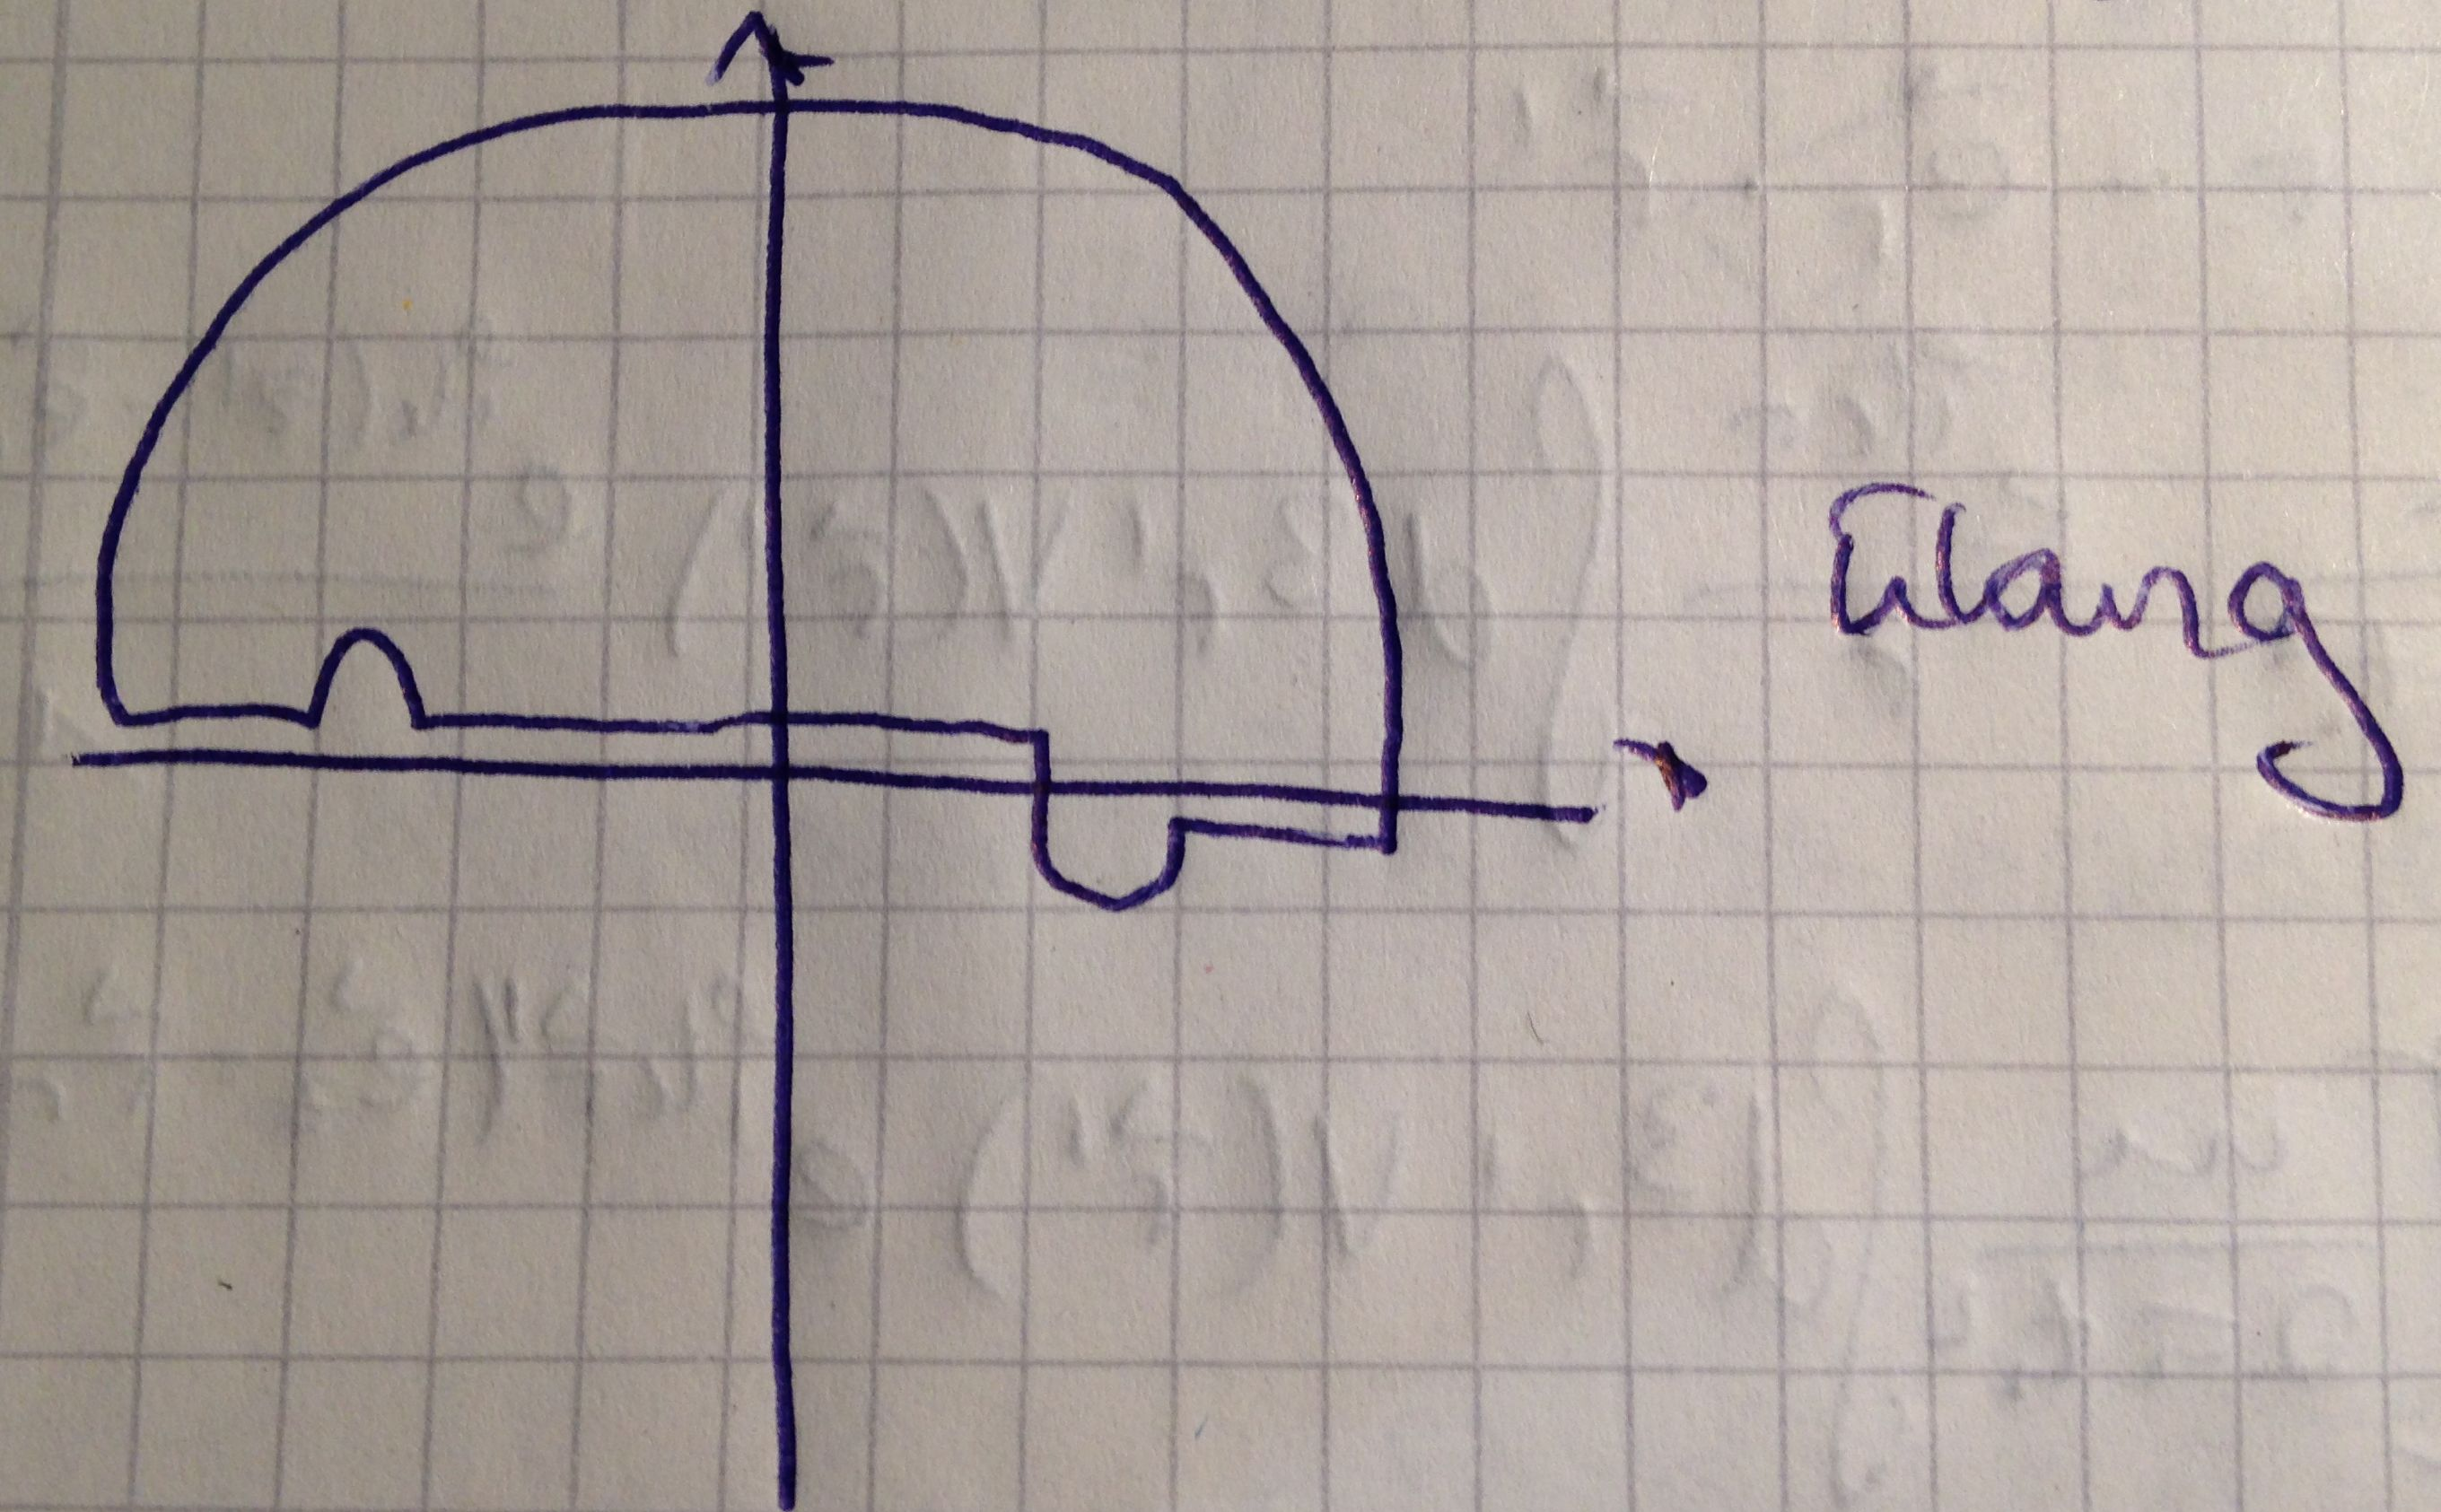
\includegraphics[width=8cm]{Born_Naeherung}
		\end{center}
	\end{figure*}
	Lösung der inhomogenen Gleichung:
		\begin{align*}
			\phi(\vec{r}) &= \phi_0 (\vec{r}) + 
			\int \diff^3 r' ~G(\vec{r} - \vec{r}\,') \frac{2m}{\hbar^2} V(\vec{r}\,') \phi (\vec{r}\,') \\
			&= \underbrace{e^{ikr \cos \theta}}_{\substack{\text{einlaufende Welle}}}
			\underbrace{- \frac{m}{2 \pi \hbar^2} \int \diff^3 r' ~V(\vec{r}\,') 
			\frac{e^{ik |\vec{r} - \vec{r}\,'|}}{|\vec{r} - \vec{r}\,'|} \phi (\vec{r}\,')}_{\mathclap{[
				B\phi] (\vec{r}) \text{ mit } ``B=\frac{2m}{\hbar^2} GV''}} 
		\end{align*}
		\begin{align*}
			\phi &= \phi_0 + B \phi &
			&\Rightarrow \phi_0 = \phi - B \phi = (1 - B) \phi \\
			\phi &= (\mathds{1} - B)^{-1} \phi_0 = \sum_{n = 0}^{\infty} B^n \phi_0 &
			&= \phi_0 + B \phi_0 + B^2 \phi_0 + \ldots \\
			& & &\text{\underline{Born-Reihe}}
		\end{align*}
	oder
		\begin{align*}
			\phi (\vec{r}) &= e^{ikr \cos \theta}
			- \frac{m}{2 \pi \hbar^2} \int \diff^3 r' ~V(\vec{r}\,') 
			\frac{e^{ik |\vec{r} - \vec{r}\,'|}}{|\vec{r} - \vec{r}\,'|}
			e^{ikr' \cos \theta'} \\
			&+ \frac{m^2}{4 \pi^2 \hbar^4} \int \diff^3 r' ~\diff^3 r'' 
			~V(\vec{r}\,') 
			\frac{e^{ik |\vec{r} - \vec{r}\,'|}}{|\vec{r} - \vec{r}\,'|}
			~V(\vec{r}\,'') 
			\frac{e^{ik |\vec{r}\,' - \vec{r}\,''|}}{|\vec{r}\,' - \vec{r}\,''|}
			e^{ikr'' \cos \theta''} \\
			&- \ldots
		\end{align*}
	1.Ordnung:
		\begin{align*}
			|\vec{r} - \vec{r}\,'| &= (r^2+r'^2 - 2 \vec{r} \vec{r}\,')^{\frac{1}{2}} 
			\overset{r \gg r'}{\approx}
			r \left(1 - \frac{2 \vec{r} \vec{r}\,'}{r^2} + \frac{r'^2}{r^2}\right)^{\frac{1}{2}}\\
			&\approx r - \frac{\vec{r} \cdot \vec{r}\,'}{r} = r - \vec{e}_r \cdot \vec{r}\,'\\
			\phi (\vec{r}) &\underset{r\rightarrow \infty}{\longrightarrow} 
			e^{ikr \cos \theta} 
			- \frac{m}{2 \pi \hbar^2} \frac{e^{ikr}}{r}
			\int \diff^3 r' ~V(\vec{r}\,') 
			\frac{e^{ik (z' - \vec{e}_r \cdot \vec{r}\,')}}{1} + \ldots \\
			&= e^{ikr \cos \theta} - \frac{e^{ikr}}{r}
			\left[ \frac{m}{2 \pi \hbar^2} \int \diff^3 r' ~V(\vec{r}\,') 
				e^{ik \vec{r}\,' (\vec{e}_r \cdot \vec{r}_r)} 
			\right] + \ldots
		\end{align*}
	\begin{minipage}{0.5\textwidth}
	Impulsübertragung
		\begin{align*}
		\vec{q} = \vec{k} - \vec{k}_0 &= \vec{k} (\vec{e}_r - \vec{e}_z) \\
		|\vec{k}_0| &= |\vec{k}|
		\end{align*}
	\end{minipage}
	\hfill
	\begin{minipage}{0.4\textwidth}
		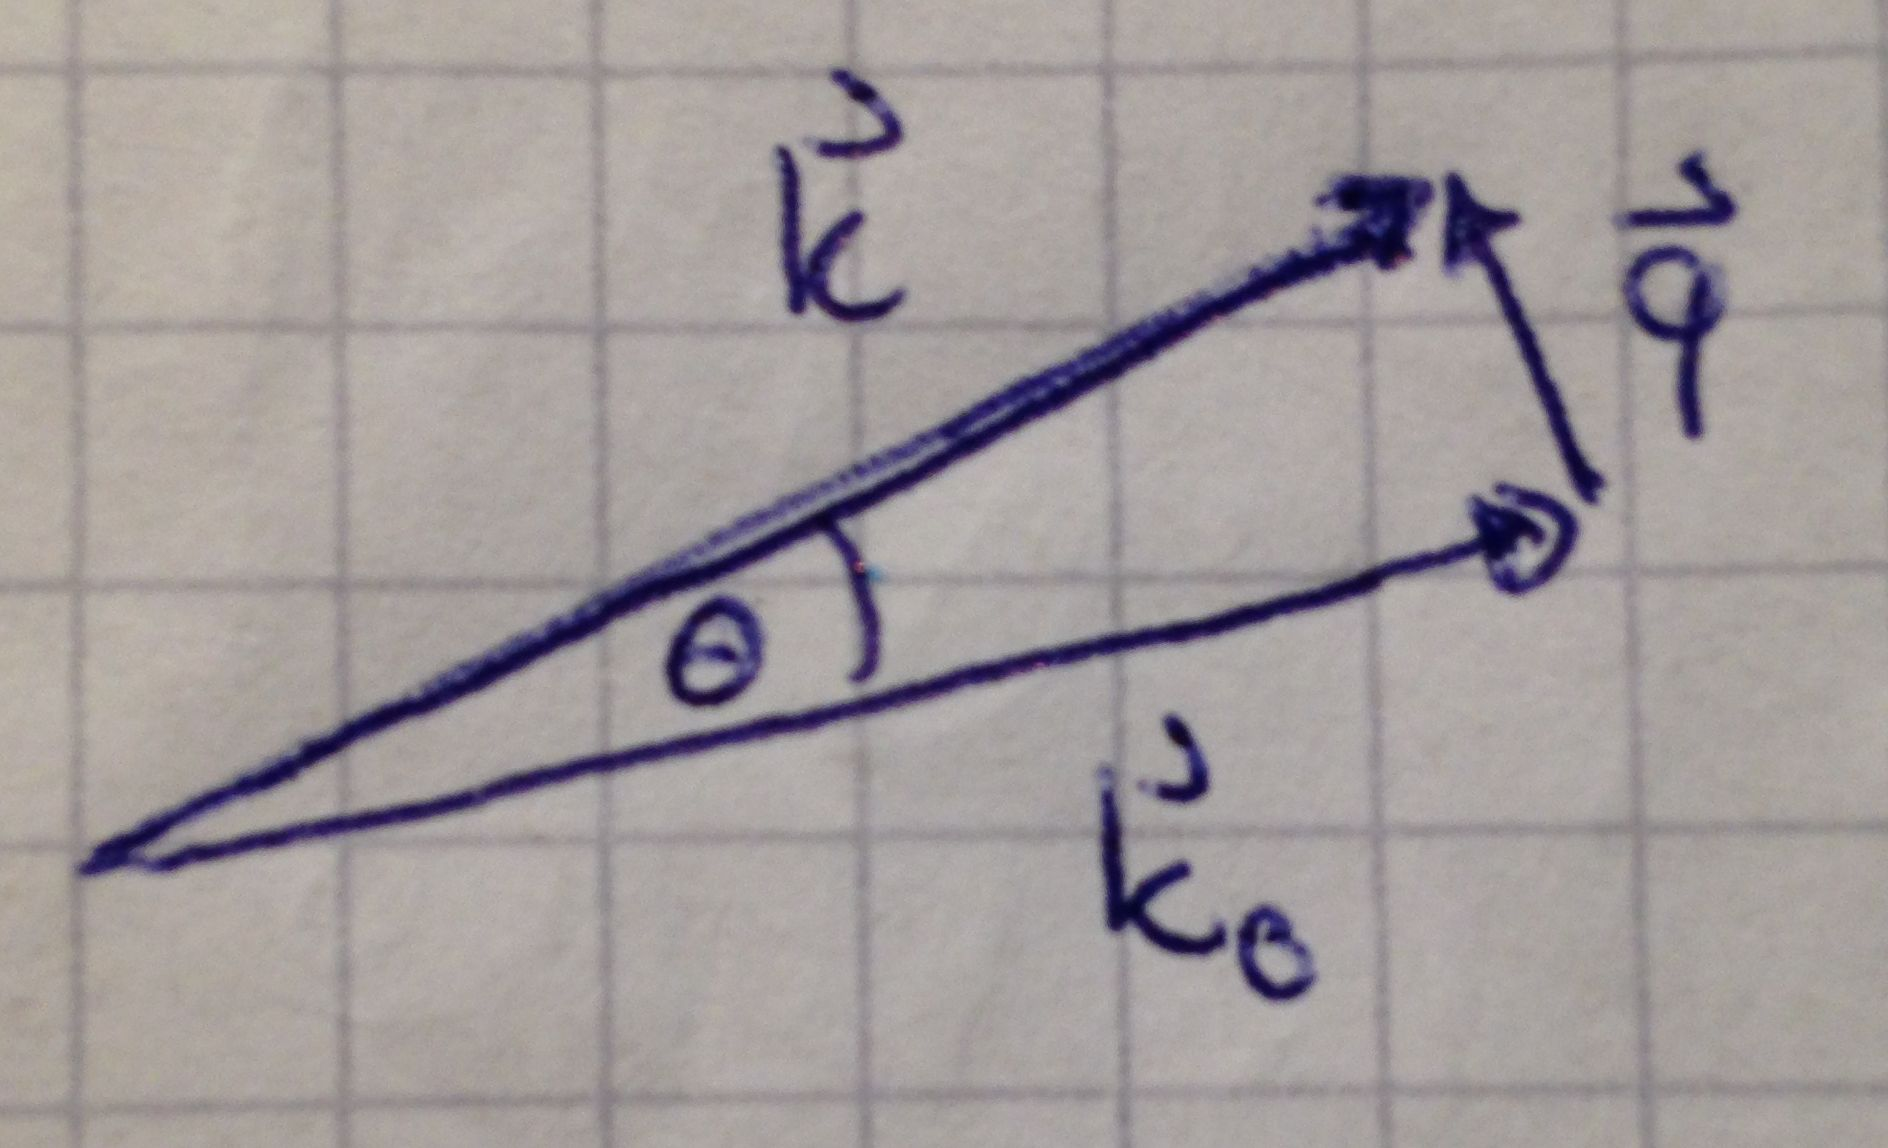
\includegraphics[width=5cm]{Born_Naeherung2}
	\end{minipage}
		
	Born-Näherung für Streuamplitude:
		\begin{empheq}[box=\boxed]{align*}
			f^{(1)} (\theta, \phi) &= -\frac{m}{2 \pi \hbar^2} 
			\int \diff^3 r' ~V(\vec{r}\,') e^{-i \vec{q} \vec{r}}
		\end{empheq}
		\begin{align*}
			f^{(1)} &= -\frac{m}{2 \pi \hbar^2}  \braket{\vec{k}| V | \vec{k}_0}
			& &V \text{ ist Wechselwirkung}
		\end{align*}
	Born-Näherung (1.Ordung der Born-Reihe) der Streuamplitude ist die Fouriertransformierte des Streupotentials.
	
	Impulsübertragung: \marginpar{12.11.2015}
		\begin{align*}
			\vec{q} &= \vec{k} - \vec{k}_0 
			= k (\vec{e}_r - \vec{e}_z)
		\end{align*}
	Wobei $k = |k| = |k_0|$

%	\begin{figure*} [h]
%		\begin{center}
%			\includegraphics[width=8cm]{Annaherung_harte_Kugel3}
%		\end{center}
%	\end{figure*} %dieses Bild hab ich nicht
	
	Born-Näherung für Streuamplitude
		\begin{empheq}[box=\boxed]{align*}
			f^{(1)}(\theta, \phi) =
			-\frac{m}{2 \pi \hbar} 
			\int \diff^3 r' ~V(\vec{r}\,') e^{-i \vec{q} \cdot \vec{r}}
		\end{empheq} 
		\begin{align*}
			``f^{(1)} = -\frac{m}{2 \pi \hbar} 
			\braket{ \vec{k} | V | \vec{k}_0}\text{''}
		\end{align*}
	Streuamplitude ist in Born-Näherung die ``Fouriertransformierte'' des Streupotetials.
	
	Annahme: Kugelsymmetrisches Streupotential:
		\begin{empheq}[box=\boxed]{align*}
			\vec{q}^2 &= (\vec{k} - \vec{k}_0)^2 
			= k^2 \left( 1 - \frac{2 \vec{k} \vec{k}_0}{k^2}
			+ 1 \right)	
			= 2 k^2 (1- \cos \theta) \\
			&= 4 k^2 \sin^2 \frac{\theta}{2}
		\end{empheq}
	wobei $k^2 = |\vec{k}| |\vec{k}_0|$
	
	Setze $\vec{q} = \left[ 4 k^2 \sin^2 \frac{\theta}{2} 
	\right]$ in Born-Näherung ein:
		\begin{align*}
			\int \diff^3 r ~V(\vec{r}\,') e^{-i \vec{q} \vec{r}}
			&= 2 \pi \int_{-\infty}^{\infty} \diff r' 
			~r'^2 V(r') 
			\underbrace{\int_{-1}^1 \diff \cos \theta 
			e^{-iqr \cos \theta}}_{\substack{*}} \\
			\left(
			*: \int_{-1}^1 \diff t ~e^{-iqr t} \right.
			\left. 
				- \frac{1}{iqr} e^{-iqrt}
			\right|_{-1}^1
			&= 
				\left. \frac{2}{qr} \sin (qr)
			\right) \\
			\int \diff^3 r ~V(\vec{r}\,') e^{-i \vec{q} \vec{r}}
			&= \frac{4 \pi}{q} \int_{0}^{\infty}
			\diff r' ~r' V(r') \sin (qr')
		\end{align*}
	Streuamplitude: \marginpar{beim zweiten bruch steht noch ein q irgendwie drunter}
		\begin{empheq}[box=\boxed]{align*}
			f^{(1)} (\theta, \phi) = f^{(1)}(\theta)
			= -\frac{2m}{\hbar^2} \frac{1}{2 k \sin \frac{\theta}{2}} 
			\int_0^{\infty} \diff r' ~r' V(r') \sin (qr')
		\end{empheq}
	Streuamplitude in Born-Näherung für rotationssymmetrische Wechselwirkung.
	
	Optisches Theorem:
		\begin{align*}
			\mathrm{Im} f(\theta = 0) &= \frac{k}{4 \pi} \sigma
			& &\text{Problem: } f^{(1)} \text{ ist reell!}
		\end{align*}
	Die Born-Näherung verletzt das optische Theorem.
	Unzuverlässig bei kleinen $\theta$. Kann nur ``funktionieren'' weg von Vorwärtsentwicklung.
	
	``Gültigkeitsbereich'' (2 Fälle):
		\begin{itemize}
			\item niedrige Energie ($kR \ll 1$):
			$| \int_0^\infty \diff r ~r V(r)|
			\ll \frac{\hbar^2}{2m}$
			\item hohe Energien ($kR \gg 1$):
			$ | \int_0^\infty \diff r ~V(r)| 
			\gg \frac{\hbar^2 k}{2m}$ 
			+ nur für $\theta > 0$
		\end{itemize}
	Beispiel: Yukawa-Potential: 
		\begin{align*}
			V(r) &= \frac{g^2}{4 \pi} \frac{e^{-\mu r}}{r}
			& &\text{Reichweite } R \sim \frac{1}{\mu} \\
			f^{(1)} (\theta) 
			&= - \frac{2m}{\hbar^2} \frac{1}{2 k \sin \left(\frac{\theta}{2}\right)} 
			\int_0^\infty \diff r' ~r' V(r')
			\sin \left(2 k \sin \frac{\theta}{r} r'\right) \\
			&= - \frac{g^2}{4 \pi} \frac{m}{\hbar k \sin \frac{\theta}{2}}
			\int_0^\infty \diff r' ~e^{-\mu r'} 
			\sin \left(2 k \sin \frac{\theta}{2} r' \right)
		\end{align*}
	2 fache partielle Integration:
		\begin{align*}
			f^{(1)}(\theta) 
			&= - \frac{g^2}{4 \pi} \frac{2m}{\hbar^2}
			\frac{1}{\mu^2 +  4 k^2 \sin^2 \frac{\theta}{2}}
			& \mu \rightarrow 0 
			&\Rightarrow \text{ Coulombpotential} \\
			\text{mit } \frac{g^2}{4 \pi} 
			&= Z_1 Z_2 \alpha \hbar c 
			& \text{und } k^2 &= \frac{2mE}{\hbar^2}
		\end{align*}
	und $Z_1$ ist Ladung von Teilen, $Z_2$ ist Ladung von Streuzentrum.
		\begin{empheq}[box=\boxed]{align*}
			\left( \frac{\diff \sigma}{\diff \Omega} \right)^{(1)} 
			&= | f^{(1)}_{\text{Coulomb}}|^2
			= \left(
				\frac{Z_1 Z_2 \alpha \hbar c}{4 E}
			\right)^2
			\frac{1}{\sin^4 \left(\frac{\theta}{2} \right)}
		\end{empheq}
	Dies ist die \underline{Rutherfordstreuung}.
	
	Wir haben ``Glück'', da
		\begin{align*}
			\underset{r \rightarrow \infty}{\lim} r ~V(r) \neq 0
		\end{align*}
	exakte Coulombamplitude unterswcheidet sich von Born-Näherung in diesem Fall nur durch eine Phase.
		\begin{align*}
			f^{\text{exakt}}_{\text{Coulomb}} (\theta) 
			&= -\frac{Z_1 Z_2 \alpha \hbar c}{4 E \sin^2 \frac{\theta}{2}} 
			\exp \left[ 2 i \sigma_0 - 
			2 i \frac{Z_1 Z_2 \alpha \hbar c}{4 E} k 
			\ln \left(\sin^2 \frac{\theta}{2} \right)
			\right] \\
			\text{Streuphase }: \sigma 
			&= \sum_\ell \sigma_\ell 
			= \frac{4 \pi}{k^2} \sum_\ell (2 \ell + 1) \sin^2 \delta_\ell
		\end{align*}
	Born-Näherung für Streuphasen $\delta_\ell$: Einlaufendes Teilen (vgl. harte Kugel)
		\begin{align*}
			e^{i \vec{k_0} \vec{r}\,'} 
			&= \sum_\ell \sqrt{4 \pi (2 \ell + 1)} 
			i^\ell j_\ell (kr') Y_{\ell 0} (\theta') \\
			e^{-i \vec{k} \vec{r}} 
			&= \sum_\ell \sum_{m = -\ell}^\ell
			4 \pi (-i)^\ell j_\ell (kr') Y_{\ell m} (\theta, \phi) Y^*_{\ell m} (\theta', \phi')
		\end{align*}
	Nebenbemerkung:
		\begin{align*}
			\sum_m Y_{\ell m} (\theta, \phi) Y^*_{\ell m} (\theta', \phi') 
			&= \frac{2 \ell + 1}{4 \pi} P_\ell (\cos \sphericalangle (\vec{r},\vec{r}\,'))
		\end{align*}
		\begin{align*}
			\Rightarrow \int \diff \Omega' 
			e^{i(\vec{k}-\vec{k}_0) \vec{r}\,'} 
			&= 4 \pi \sum_{\ell=0}^\infty (2\ell + 1)
			P_\ell (\cos \theta) j_\ell^2 (kr') \\
			f^{(1)} (\theta) 
			&= -\frac{m}{2 \pi \hbar^2} 
			\int \diff^3 r' V(r') e^{i(\vec{k}-\vec{k}_0)\vec{r}} \\
			&= - \frac{2 m}{\hbar^2}
			\int \limits_0^r \diff r' ~r'^2 V(r') 
			\sum_{\ell = 0}^\infty j_\ell^2 (k r') 
			(2 \ell + 1) P_\ell (\cos \theta) 
		\end{align*}
	Vergleich mit:
		\begin{align*}
			f^{(1)}(\theta) 
			&= \frac{1}{k} \sum_{\ell=0}^{\infty} (2\ell + 1)
			\underline{e^{i\delta_\ell} \sin \delta_\ell} P_\ell (\cos \theta) \\
			\Rightarrow e^{i\delta_\ell} \sin \delta_\ell
			&= - \frac{k 2 m}{\hbar^2} 
			\int \limits_0^\infty \diff r ~V(r) 
			[r ~j_\ell(kr)]^2
		\end{align*}
	Streuphasen für rotationssymmetrisches Potential in Born-Näherung:
		\begin{empheq}[box=\boxed]{align*}
			\mathrm{Re} (\underline{ e^{i\delta_\ell} \sin \delta_\ell})
			&\approx \delta_\ell
			\leftarrow \delta_\ell \text{ klein für Born-Näherung} \\
			&\approx -\frac{2m}{k \hbar^2}
			\int \limits_0^\infty \diff r ~V(r) 
			~[(kr)j_\ell(kr)]^2
		\end{empheq}